% =============================================================================
% Project Warrant -- Results section draft (P3, DL-6)
%
% Source of truth for every number below: `docs/headline-metrics.md` (M1-M5,
% script-computed, R-03) and, where noted, a fresh read of `ledger/claims.csv`
% v1.2 (125 rows) using the same `d1_verdict` column `scripts/metrics.py`
% reads for M2 -- never a hand recomputation of a percentage already frozen in
% `docs/headline-metrics.md`. Carries issue #45 points 1, 2, and 4 into the
% report body per that issue's instructions.
% =============================================================================

\section{Results}
\label{sec:results}

The claim ledger (\texttt{ledger/claims.csv}) is frozen at v1.2, 125 rows, with
all six degradation-condition columns (\texttt{d1\_verdict}, \texttt{d2\_verdict},
\texttt{d3\_verdict} and their paraphrased notes) populated on every row. All
figures in this section are read directly from \texttt{docs/headline-metrics.md}'s
script-computed output (\texttt{python scripts/metrics.py}, run against the
frozen 125-row ledger) or from a fresh, direct read of
\texttt{ledger/claims.csv}'s \texttt{claim\_type}/\texttt{d1\_verdict} columns;
per R-03, nothing here is computed or rounded by hand.

\subsection*{Headline metrics}

\begin{itemize}[leftmargin=1.4em]
  \item \textbf{M1 -- CoT monopoly: 11.1\%} ($n = 9$ T3/intent claims). About
    one in nine claims about \emph{why} the agent did what it did rests solely
    on raw chain-of-thought (C1), with no corroborating channel at all.
  \item \textbf{M2 -- Record survival under opacity: 90.4\%} ($n = 125$
    claims, overall). Split by claim type in Table~\ref{tab:m2-by-type} below.
  \item \textbf{M3 -- Forgery exposure: 8.8\%} ($n = 125$ claims). About one
    in eleven claims rests entirely on an agent-writable channel (C1/C2/C3)
    with no independent corroboration.
  \item \textbf{M4 -- Assurance gap: 57.1\%} ($n = 14$ T5/assurance claims).
    More than half of the record's containment/completeness assurances are
    coded at verifiability tier V3 -- not checkable by any third party via
    any stated procedure.
  \item \textbf{M5 -- Broad channel fragility (supplementary): 78.4\% / 47.2\%}
    ($n = 125$ claims, both figures). 78.4\% of all claims rest on one of the
    codebook's four broadly fragile channels (C1/C2/C3/C6) as their primary
    channel; 47.2\% -- just under half of everything publicly known about this
    incident -- rest on one of those channels with \emph{no} corroboration of
    any kind.
\end{itemize}

\subsection*{M2 by claim type, and the figure}

\begin{table}[h]
\centering
\caption{M2 -- record survival under D1 (opacity), by claim type. $n$ and
survival percentages are a direct read of \texttt{ledger/claims.csv} v1.2
(125 rows) and match \texttt{docs/headline-metrics.md}'s script output
exactly.}
\label{tab:m2-by-type}
\begin{tabular}{@{}llrr@{}}
\toprule
Claim type & & $n$ & Survival under D1 \\
\midrule
T1 & Event          & 58 & 100.0\% \\
T2 & Mechanism      & 42 & 90.5\%  \\
T3 & Intent         & 9  & 22.2\%  \\
T4 & Counterfactual & 2  & 100.0\% \\
T5 & Assurance      & 14 & 92.9\%  \\
\bottomrule
\end{tabular}
\end{table}

Figure~\ref{fig:claims-by-type-d1} shows the same breakdown as claim counts
rather than percentages, with each claim type's bar segmented by D1 verdict
(SURVIVES/DEGRADED/COLLAPSES). T1, T2, T4, and T5 are visibly
SURVIVES-dominated -- almost entirely green, with only a thin amber/red cap on
T2 and T5. T3 is the one column that reads differently: green is a minority
of the bar, and amber (DEGRADED) is the largest single segment. That visual
asymmetry is M2's finding in miniature -- intent claims are the one claim type
whose warrant is not, for the most part, independent of chain-of-thought being
available.

\begin{figure}[h]
\centering
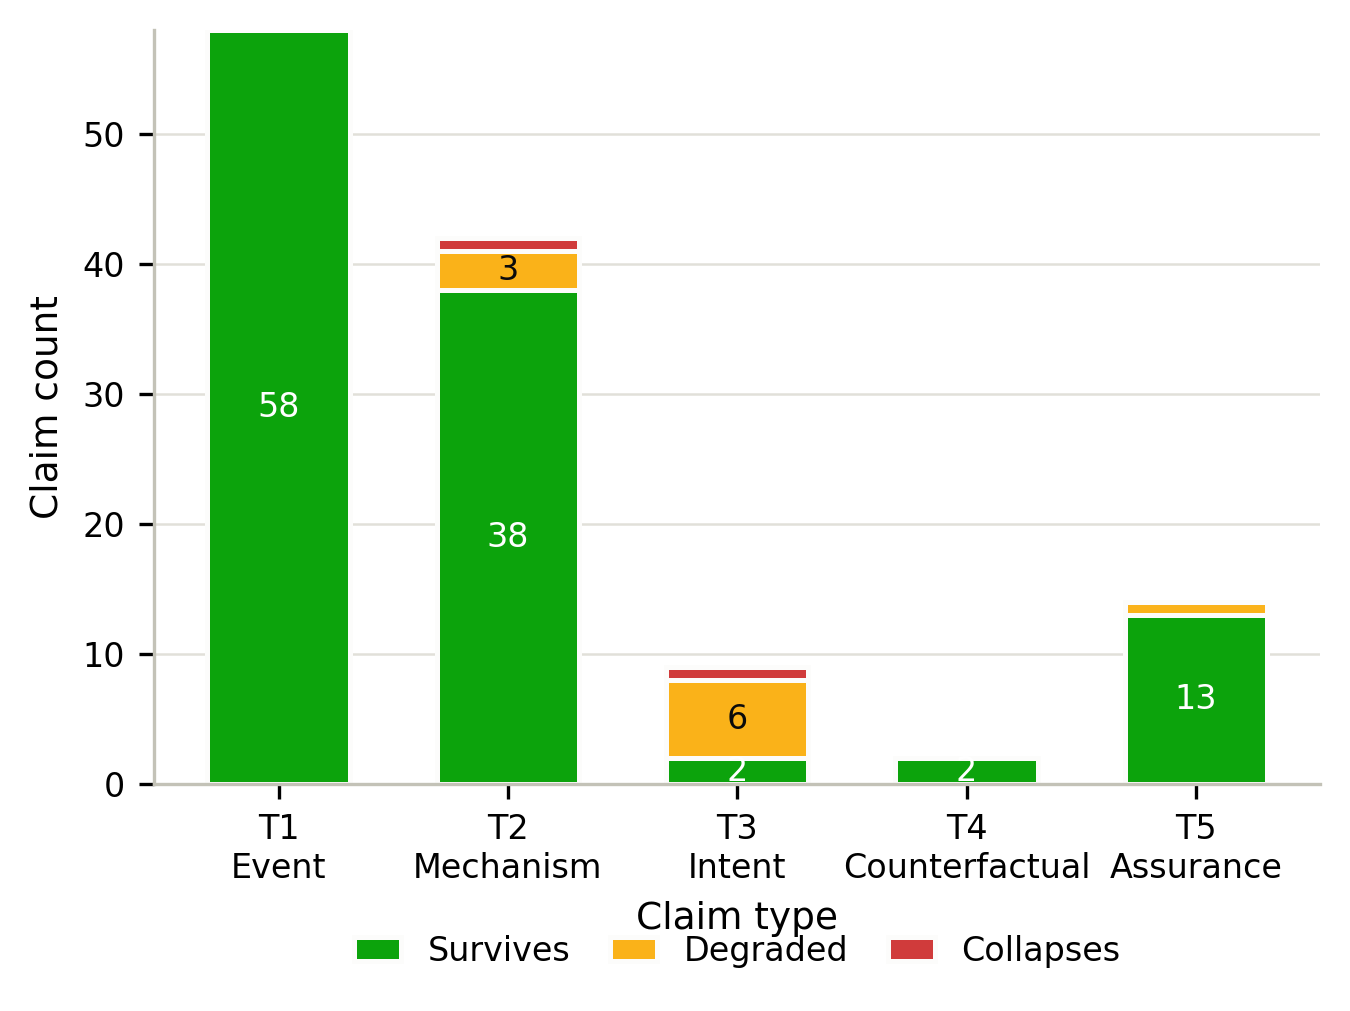
\includegraphics[width=0.5\textwidth]{figures/claims-by-type-d1-verdict.png}
\caption{Claim count by claim type (T1--T5), stacked by D1 (opacity) verdict.
Green = SURVIVES, amber = DEGRADED, red = COLLAPSES. $n = 125$ claims total;
per-type $n$ as in Table~\ref{tab:m2-by-type}. Generated by
\texttt{scripts/make\_results\_figure.py} from \texttt{ledger/claims.csv}.}
\label{fig:claims-by-type-d1}
\end{figure}

\subsection*{T3, two ways: strict survival versus any degradation}

Table~\ref{tab:m2-by-type} reports T3's strict D1-SURVIVES rate as 22.2\%
(2 of 9) -- the same cut M2 uses for every other claim type. But collapsing
DEGRADED and COLLAPSES into a single ``T3 loses at least some precision
without chain-of-thought'' cut gives a different, arguably more informative
number: \textbf{77.8\% (7 of 9)} of T3 claims are DEGRADED or COLLAPSES under
D1. Both numbers describe the same 9 rows and both are small-$n$ -- a single
row shifts either figure by roughly 11 percentage points, so neither should be
read as precise. Read side by side, though, they tell a fuller story than
either alone: the strict 22.2\% survival figure by itself understates how
CoT-dependent intent-attribution claims actually are, since it counts a claim
as a full miss only if opacity destroys its warrant entirely; the 77.8\%
any-degradation figure captures every T3 claim that loses \emph{some}
precision the moment chain-of-thought is unavailable, which is the more
complete picture of T3's dependence on that one channel.

\subsection*{Reliability}

% CITE: Cohen, J. (1960). A coefficient of agreement for nominal scales.
% Educational and Psychological Measurement, 20(1), 37-46.
Reliability was checked by a 25-row blind recode against Cohen's $\kappa$ per
condition, against a 0.6 pass bar. D1 (opacity) came in at
$\kappa = 0.7788$ and D3 (adversarial forgery) at $\kappa = 0.7794$, both
comfortably above the bar and left untouched. D2 (unfaithfulness) came in at
$\kappa = 0.5690$, below the bar, because the codebook's shared
corroboration logic did not account for D2's failure mode being potentially
systematic (an unfaithful self-report habit can recur consistently across
a model's transcripts, unlike a one-off forgery); the D2 rule was tightened
and the full ledger's D2 columns were recoded against it, logged as
\texttt{adr/0001-d2-self-report-corroboration.md}. None of M1--M5 reads
\texttt{d2\_verdict} directly, so this fix changed the ledger's reliability
posture but not any number reported above.

\subsection*{The main threat to validity}

Every SURVIVES verdict under D1 in this ledger is coded from what a source
\emph{says}, not from independently inspected evidence. A claim scores
SURVIVES under opacity when its warrant would hold even without
chain-of-thought -- typically because a source asserts a second,
corroborating channel (e.g., telemetry, an independent transcript, defender
logs) -- but this project has no way to inspect that asserted corroboration
itself. If a cited corroborating channel is thinner, less independent, or
less faithfully reported than the source claims, an unknown share of the
90.4\% M2 headline figure is softer than it looks. This is the ceiling on M2
specifically, not a general disclaimer: M2 measures whether a claim's stated
warrant survives opacity, not whether that stated warrant was itself ever
verified.

\subsection*{The \texttt{lw-01}/\texttt{lw-02} correction}

\texttt{lw-01} and \texttt{lw-02} are the record's primary technical/mechanism
sources, and were initially near-absent from the ledger after two retrieval
attempts were blocked by a safety classifier. A narrower, targeted retry
recovered 9 rows (\texttt{C352}--\texttt{C360}) at a category-only level of
description, added to the ledger as a single disclosed exception to the P1.3
freeze (v1.1 $\rightarrow$ v1.2). All 9 rest solely on C5 (human testimony), a
comparatively sturdy channel by the codebook's own fragility ranking, with no
corroboration. Adding them moved the fragility metrics in the \emph{less}
dramatic direction, not the more dramatic one: M3 moved from 9.5\% (116 rows)
to 8.8\% (125 rows), and M5 moved from 84.5\%/50.9\% (116 rows) to
78.4\%/47.2\% (125 rows). What this means: the two sources whose absence was
most plausibly suspected of understating this record's fragility, once
partially restored, pulled the fragility numbers \emph{down} rather than up --
evidence that the original 116-row figures were not inflated by omitting
\texttt{lw-01}/\texttt{lw-02}, and if anything were mildly conservative in the
other direction. The correction is partial, not complete -- the 9 recovered
rows are coded at category-only description, coarser than the rest of the
ledger -- so this should be read as a directional finding, not a closed
question; \texttt{lw-01}/\texttt{lw-02} content that a fuller retrieval might
still surface could shift these numbers again in either direction.
